\chapterhead{\centering CHƯƠNG 2 $-$ PHÂN TÍCH THIẾT KẾ HỆ THỐNG}
\addcontentsline{toc}{chapter}{CHƯƠNG 2 $-$ PHÂN TÍCH THIẾT KẾ HỆ THỐNG}

\section*{2.1 Tóm tắt hệ thống}
\addcontentsline{toc}{section}{2.1 Tóm tắt hệ thống}

Trong bài báo này, sẽ triển khai hệ thống mạng cho Công Ty TNHH Công Nghệ SmartTech, bao gồm việc cài đặt cân bằng băng tải, tính khả dụng cao và khả năng mở rộng trong tương lai. Thiết kế hệ thống với các thành phần chính như Router, Switch, Server và các PC.

\textbf{Các giai đoạn thực hiện:}

- Giai đoạn 1: Khảo sát và phân tích
\begin{itemize}[left=2.5cm]
    \item Khảo sát địa điểm, bố trí mặt bằng và hệ thống điện.
    \item Thực hiện phân tích, tính toán lưu lượng băng thông, dự phòng và khả năng mở rộng trong tương lai.
    \item Chọn thiết bị mạng và cách bố trí.
    \item Đảm bảo hệ thống đáp ứng yêu cầu của công ty đưa ra.
\end{itemize}

- Giai đoạn 2: Thiết kế
\begin{itemize}[left=2.5cm]
    \item Phác thảo sơ đồ luận lý và sơ đồ vật lý của hệ thống mạng.
    \item Đảm bảo cấu hình vật lý của thiết bị đảm bảo kết nối và hiệu suất tối ưu cho hệ thống mạng.
\end{itemize}

- Giai đoạn 3: Triển khai, cấu hình và thực nghiệm
\begin{itemize}[left=2.5cm]
    \item Triển khai hệ thống dựa trên sơ đồ đã được hoàn thiện.
    \item Cấu hình các thiết bị mạng đã triển khai.
    \item Kiểm thử hệ thống để đảm bảo hệ thống hoạt động ổn định và đáp ứng các yêu cầu và sẵn sàng cho công việc thực tế.
\end{itemize}

Các bước kiểm thử nhằm đảm bảo hệ thống hoạt động an toàn và phát hiện kịp thời để khắc phục các vấn đề tiềm ẩn của hệ thống.
\section*{2.2 Phân tích yêu cầu của công ty}
\addcontentsline{toc}{section}{2.2 Phân tích yêu cầu của công ty}

\subsection*{2.2.1 Sơ đồ cấu trúc công ty}
\addcontentsline{toc}{subsection}{2.2.1 Sơ đồ cấu trúc công ty}

\textbf{\textit{Mặt cắt bằng từng tầng của công ty}}

\begin{figure}[htbp]
    \centering
    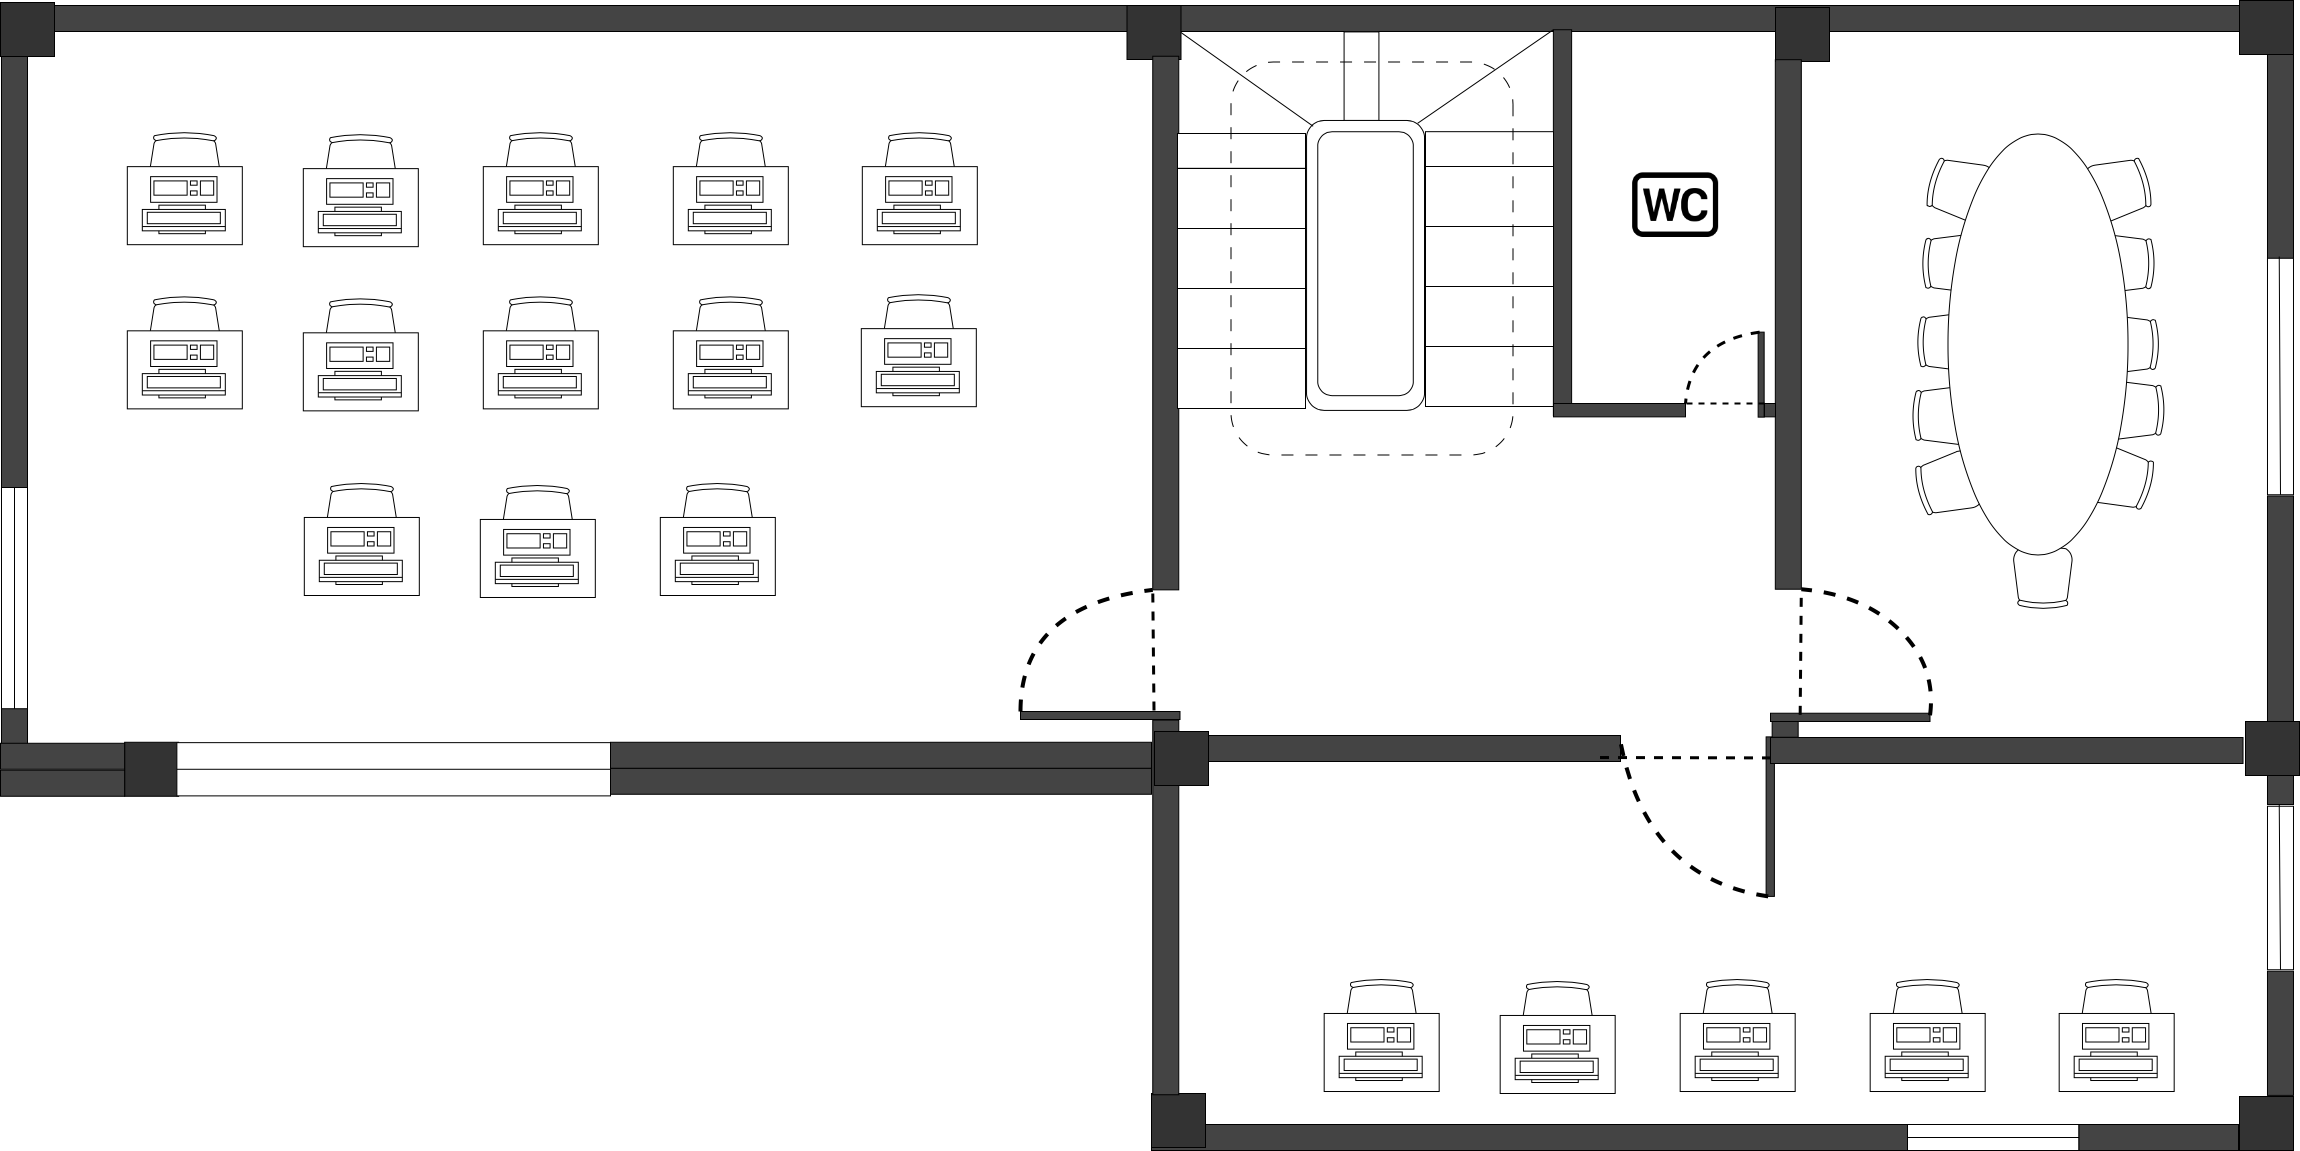
\includegraphics[width=0.6\linewidth]{img/floor1.png}
    \caption{Mặt cắt của tầng 1}
    \vspace{1cm}
    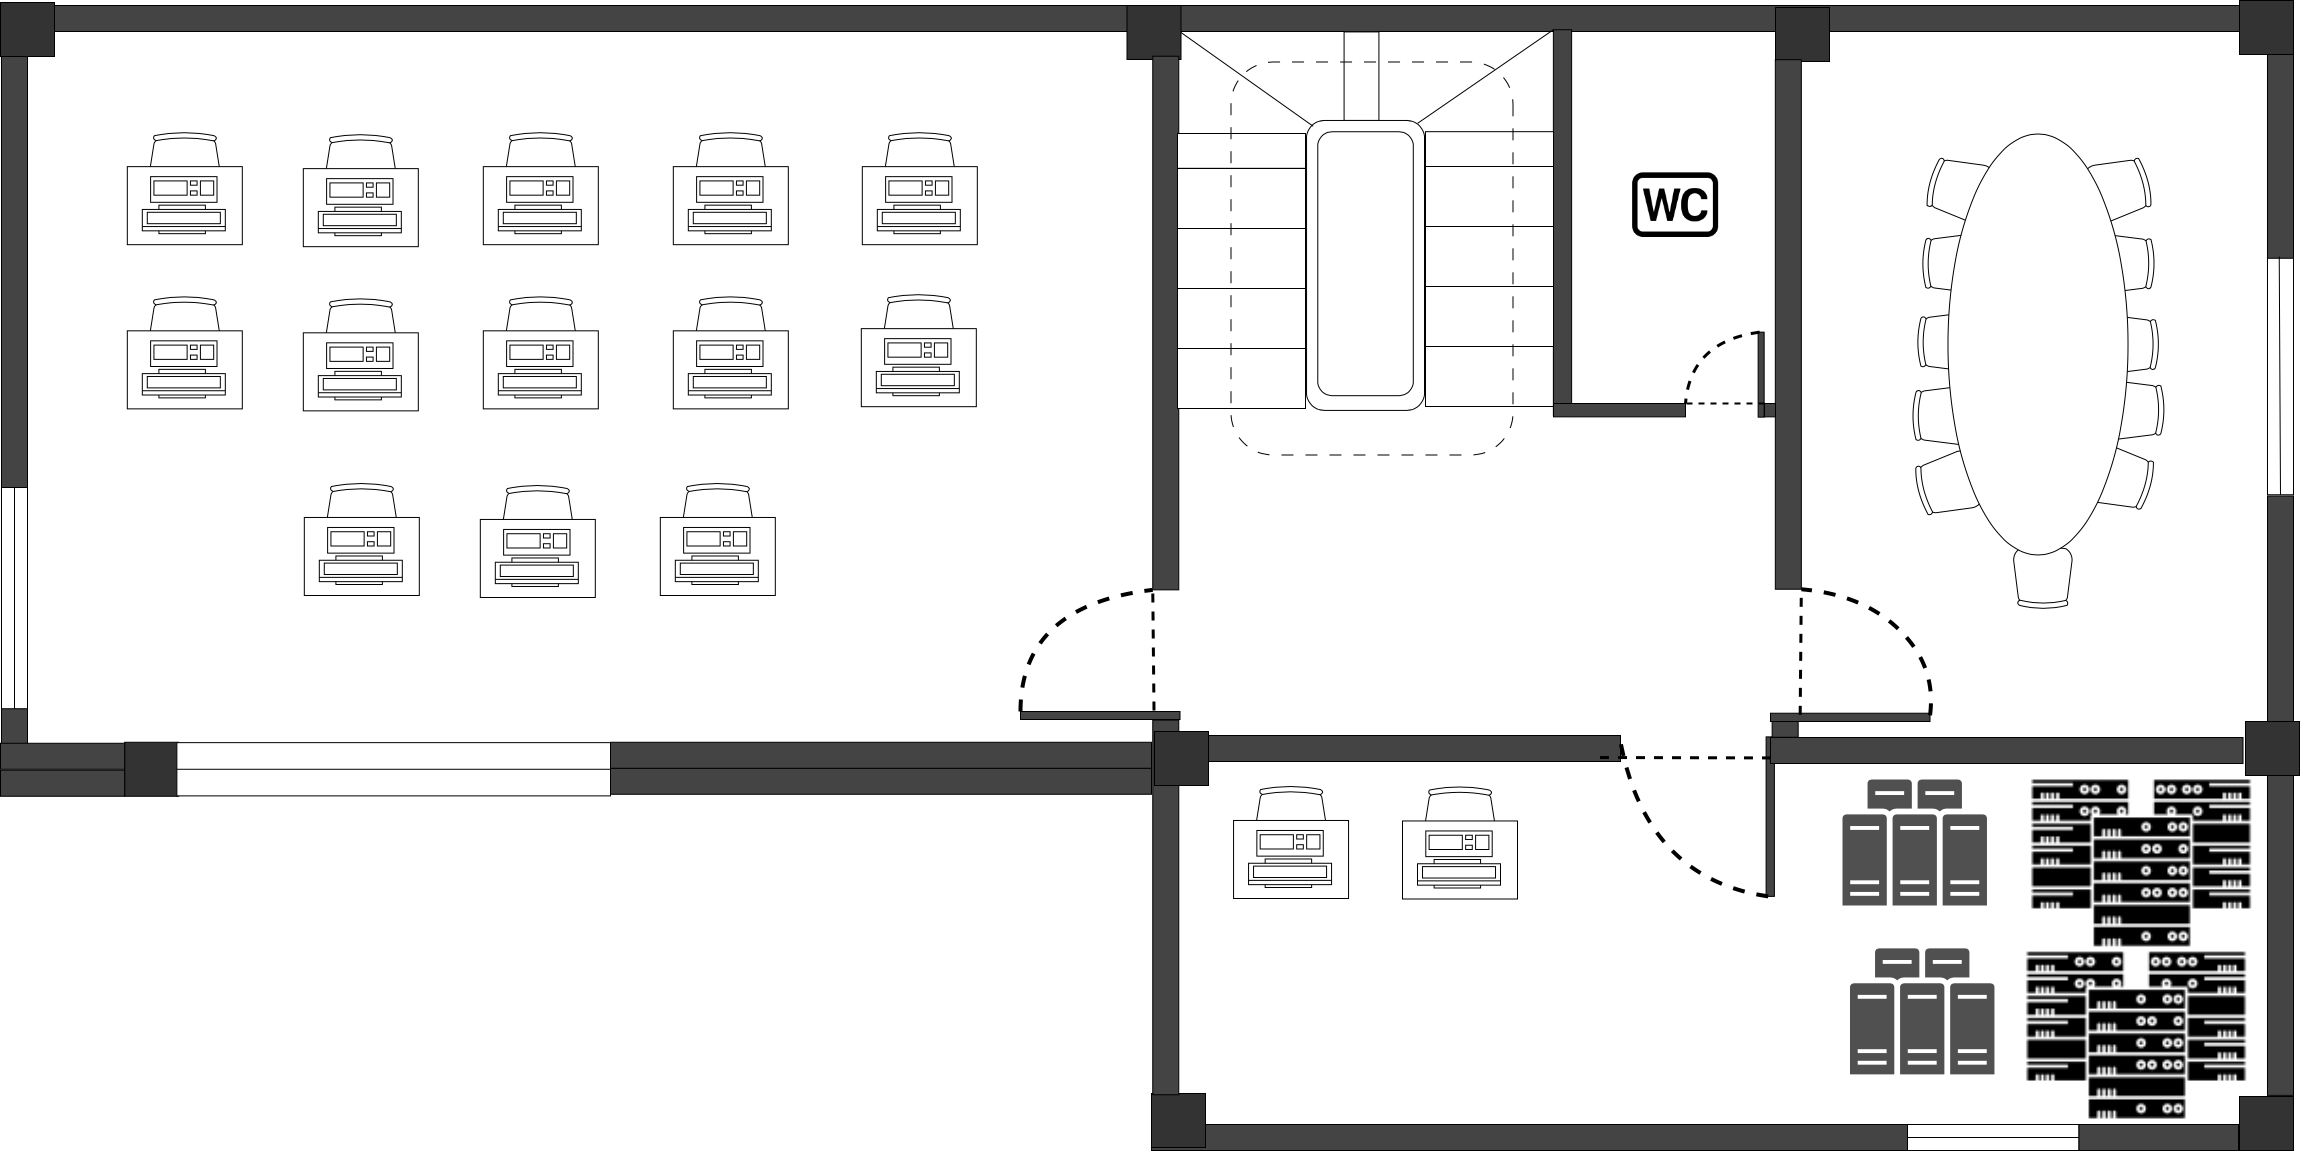
\includegraphics[width=0.6\linewidth]{img/floor2.png}
    \caption{Mặt cắt của tầng 2}
    \vspace{1cm}
     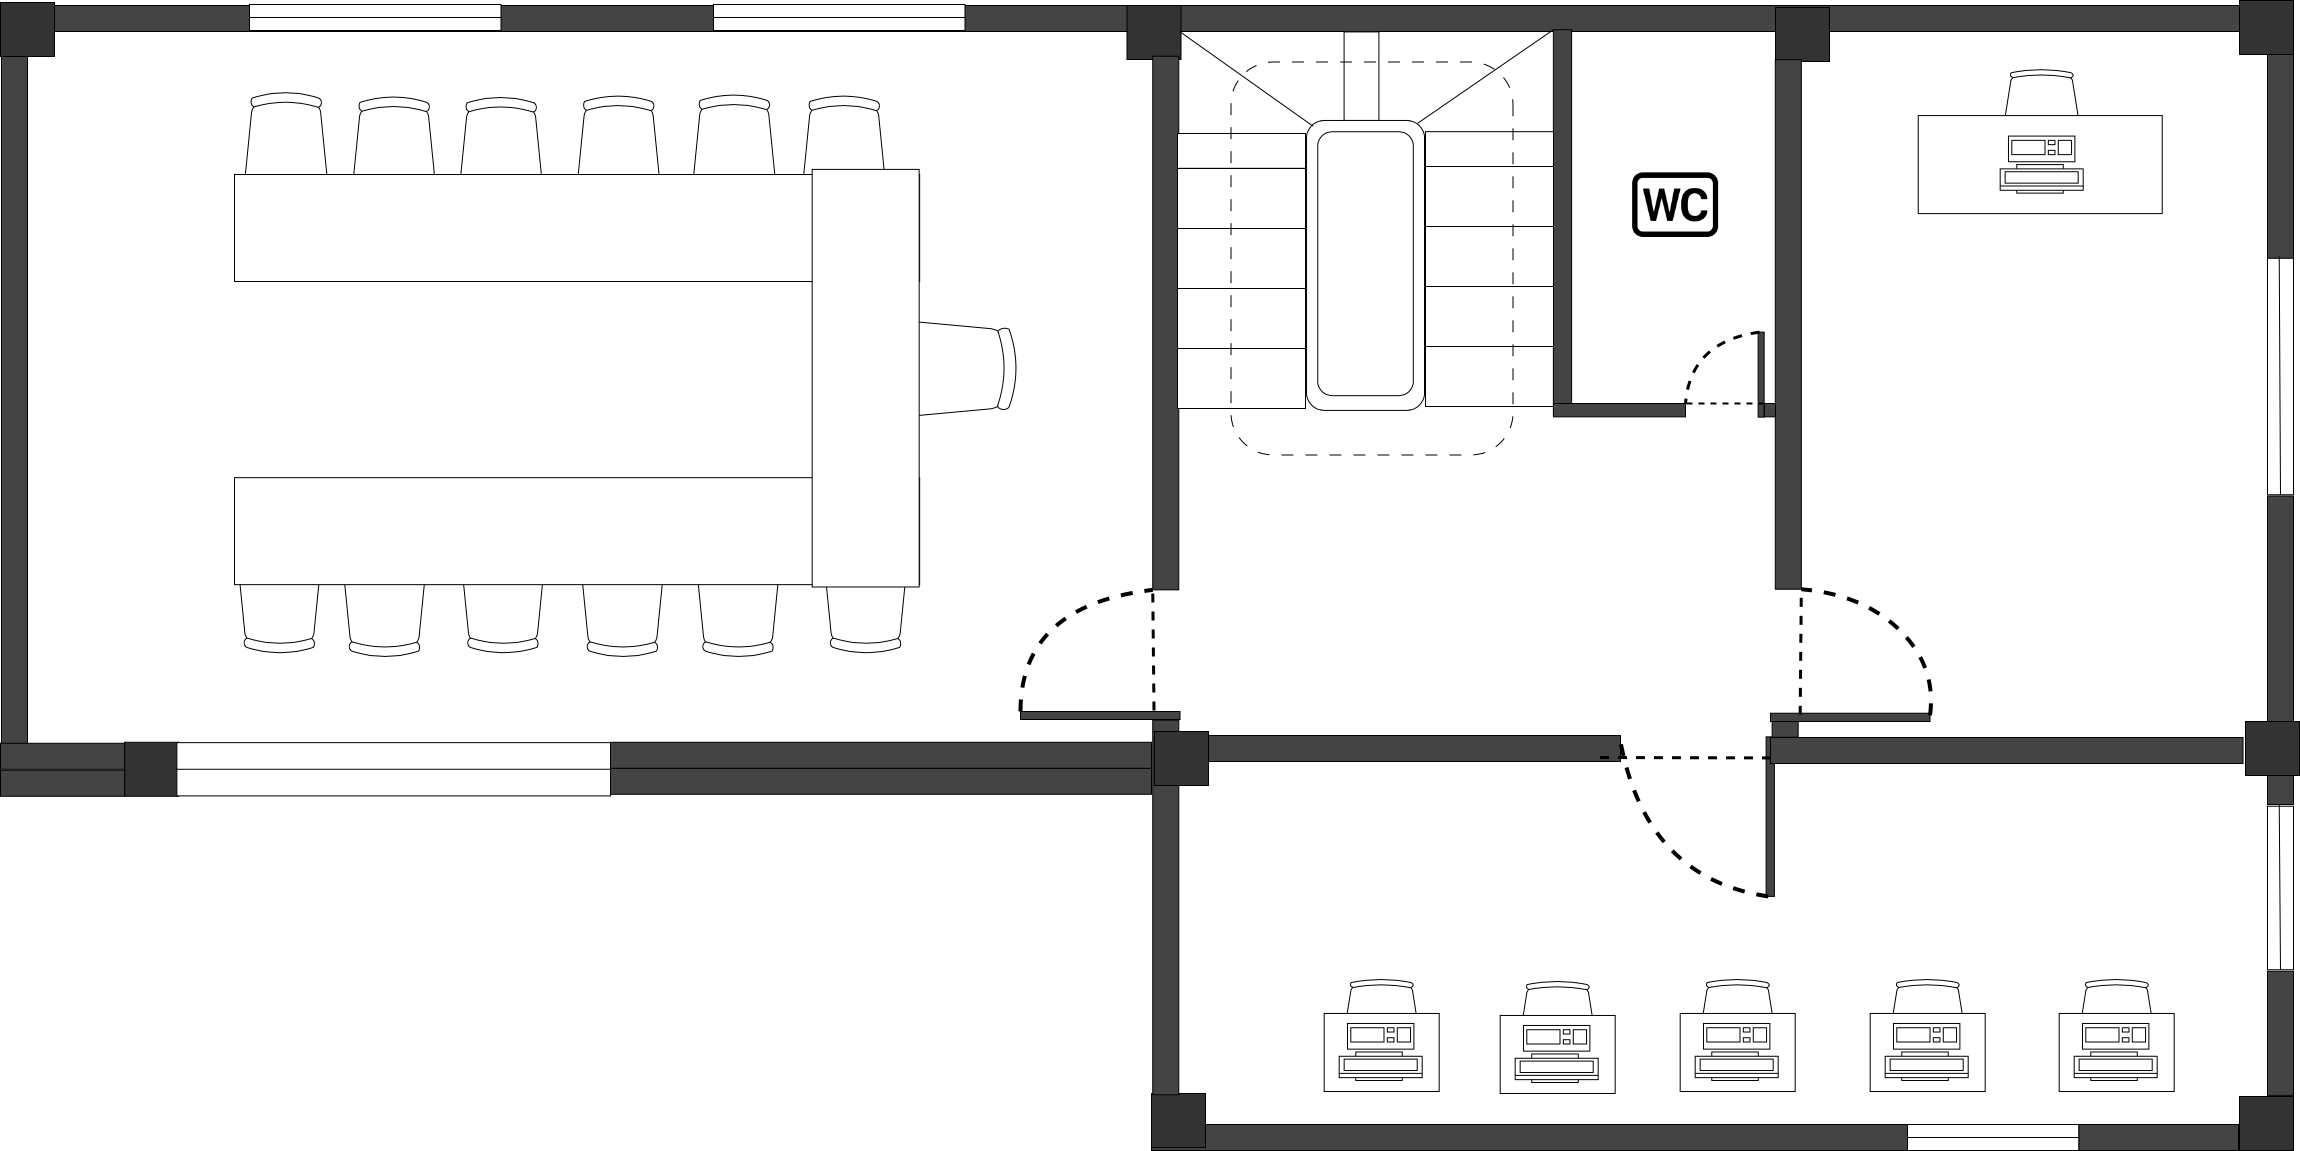
\includegraphics[width=0.6\linewidth]{img/floor3.png}
    \caption{Mặt cắt của tầng 3}
\end{figure}
\newpage
\textbf{\textit{Quy mô hệ thống}}  

Công ty Công nghệ SmartTech đặt trụ sở trong một tòa nhà có 3 tầng, với mỗi tầng được thiết kế để đáp ứng những chức năng và nhu cầu khác nhau của công ty.
 
\textbf{- Tầng 1:} Kinh doanh và chăm sóc khách hàng
   \begin{itemize}[left=2.5cm]
    \item Phòng Kinh doanh: 25 nhân viên, chịu trách nhiệm tiếp thị, giao dịch và phát triển khách hàng.
    \item Phòng Chăm sóc khách hàng: 10 nhân viên, hỗ trợ kỹ thuật và tư vấn cho khách hàng.
    \item Phòng họp nhỏ cho các cuộc họp nhóm hoặc của từng ban.
\end{itemize}

\textbf{- Tầng 2:} Phòng kỹ thuật và Trung tâm dữ liệu
   \begin{itemize}[left=2.5cm]
    \item Phòng Kỹ thuật: 40 nhân viên, đảm nhận phát triển phần mềm, triển khai dự án và hỗ trợ kỹ thuật.
    \item Trung tâm dữ liệu: Phòng riêng biệt, được thiết kế để bảo vệ an toàn và có hệ thống làm mát tốt.
    \item Phòng họp nhỏ cho các cuộc họp nhóm hoặc của từng ban.
\end{itemize}

\textbf{- Tầng 3:} Khu vực lãnh đạo
   \begin{itemize}[left=2.5cm]
    \item Văn phòng Giám đốc: Văn phòng riêng cho giám đốc công ty.
    \item Văn phòng quản lý: gồm có 4 quản lý cấp cao.
    \item Phòng họp lớn cho các cuộc họp toàn công ty hoặc hội nghị.
\end{itemize}
\subsection*{2.2.2 Phân tích yêu cầu }
\addcontentsline{toc}{subsection}{2.2.2 Phân tích yêu cầu }
\textbf{\textit{Yêu cầu cơ bản về hệ thống}}
\begin{itemize}[left=2.5cm]
    \item Yêu cầu dùng công nghệ mới về hạ tầng mạng.
    \item Tổ chức hệ thống mạng theo VLAN: Chia nhỏ mạng cho các phòng ban, các máy tính trong mỗi mạng VLAN có thể truy cập lẫn nhau.
    \item Triển khai cấu hình VPN để có thể làm việc, truy cập dự liệu đến công ty khách hàng, đối tác.
\end{itemize}

\textbf{\textit{Yêu cầu người dùng}}
\begin{itemize}[left=2.5cm]
    \item Độ tin cậy cao: Mạng phải hoạt động liên tục không có thời gian chết, ổn định vào giờ cao điểm.
    \item Hiệu suất cao: Mạng phải duy trì tốc độ truyền tải ổn định.
    \item Khả năng mở rộng: Hệ thống mạng đảm bảo có khả năng hệ thống mở rộng trong tương lai là 50\%.
    \item Dễ dàng quản lý: Hệ thống quản lý đơn giản nhưng mang lại hiệu quả cao.
    \item Bảo mật: Bảo vệ hệ thống khỏi các cuộc tấn công và truy cập mạng trái phép.
\end{itemize}

\subsection*{2.2.3 Giải pháp cho công ty}
\addcontentsline{toc}{subsection}{2.2.3 Giải pháp cho công ty}

Từ những yêu cầu trên, nhóm đã đề xuất các giải pháp sau để có thể thoả mãn các yêu cầu.
\begin{itemize}[left=2.5cm]
    \item Toàn mạng của công ty chia thành 5 VLAN cho từng phòng ban. Mỗi tầng lựa chọn số lượng switch phù hợp để có thể mở rộng số lượng máy khi cần thiết.
    \item Sử dụng ACL để kiểm soát truy câp giữa các VLAN.
    \item Sử dụng các kỹ thuật và cơ chế phân cụm chuyển đổi dự phòng.
    \item Sử dụng các phương pháp cân bằng tải để phân chia đều lưu lượng tải trên các thiết bị mạng. Giúp tăng cường hiệu suất và tránh đường các trường hợp bị quá tải trong giờ cao điểm.
    \item Cài đặt các dịch vụ mạng như DNS, Mail, Web, Data Server,... để quản lý miền trang web, chia sẻ dữ liệu, giao tiếp, chuyển mail thuận tiện hơn. 
\end{itemize}

\subsection*{2.2.4 Tính toán thông số}
\addcontentsline{toc}{subsection}{2.2.4 Tính toán thông số }
Công ty yêu cầu các ứng dụng cơ bản được cài đặt trên từng máy tính cho từng phòng ban. Dưới đây là bảng yêu cầu băng thông tối thiểu của từng ứng dụng đó:

\begin{table}[h]
    \centering
    \begin{tabular}{|l|l|l|l|}
        \hline
        \textbf{Tầng} & \textbf{Phòng} & \textbf{Ứng dụng} & \textbf{Băng thông yêu cầu} \\
        \hline
        1 & Kinh doanh & CRM & 2 Mbps/người \\
        & & Microsoft Office Online & 2 Mbps/người \\
        & & Email doanh nghiệp & 1 Mbps/người \\
        & & Phần mềm quản lý hợp đồng & 2 Mbps/người \\
        \cline{2-4}
        & Chăm sóc KH & Help Desk & 2 Mbps/người \\
        & & Remote Support & 3 Mbps/người \\
        & & CRM & 2 Mbps/người \\
        & & VoIP/Softphone & 0.1 Mbps/người \\
        \hline
        2 & Kỹ thuật & IDE & 5 Mbps/người \\
        & & Git operations & 2 Mbps/người \\
        & & Docker/Kubernetes & 10 Mbps \\
        & & Jira/Confluence & 2 Mbps/người \\
        & & Postman/API testing & 5 Mbps/người \\
        & & System monitoring & 2 Mbps \\
        & & Database tools & 5 Mbps \\
        & & VM Software & 10 Mbps \\
        & & Security tools & 2 Mbps \\
        \cline{2-4}
        & Trung tâm dữ liệu & Server monitoring & 10 Mbps \\
        & & Backup operations & 50 Mbps \\
        & & Security monitoring & 10 Mbps \\
        & & Network monitoring & 5 Mbps \\
        \hline
        3 & Lãnh đạo & Microsoft Office & 2 Mbps/người \\
        & & Project Management & 2 Mbps/người \\
        & & BI tools & 5 Mbps \\
        & & Email & 1 Mbps/người \\
        \hline
    \end{tabular}
    \caption{Yêu cầu băng thông tối thiểu cho từng ứng dụng theo phòng ban}
    \label{tab:bandwidth}
\end{table}
Với khả năng mở rộng trong tương lai là 50\% và thời gian nhân viên sử dụng tập trung là 80\%. Nhóm đã tính được băng thông yêu cầu tối thiểu, lưu lượng sử dụng thực tế và độ trễ khi truyền dữ liệu.
\newpage
\textit{\textbf{Tính băng thông cho từng tầng}}

Băng thông yêu cầu cho mỗi phòng sẽ được tính theo công thức:
\begin{equation}
    \text{Băng thông = Số người × Tổng băng thông của các ứng dụng}
\end{equation}

\textbf{Tầng 1:}
\begin{itemize}[left=2cm]
    \item Phòng Kinh doanh = 25 × (2 + 2 + 1 +  2) = 175 Mbps
    \item Phòng CSKH = 10 × (2 + 3 + 2 + 0.1) = 71 Mbps
    \item Tổng băng thông tầng 1 = 175 + 71 = 246 Mbps
\end{itemize}

\textbf{Tầng 2:}
\begin{itemize}[left=2cm]
    \item Phòng Kỹ thuật \\= 40 × (5 + 2 + 2 + 5) + 10 + 2 + 5 + 10 + 2 = 589 Mbps
    \item TTDL = 10 + 50 + 10 + 5 = 75 Mbps
    \item Tổng băng thông tầng 2 = 589 + 75 = 664 Mbps
\end{itemize}

\textbf{Tầng 3:}
\begin{itemize}[left=2cm]
    \item Phòng Giám đốc và Quản lý = 5 × (2 + 2 + 1) + 5 = 30 Mbps
    \item Tổng băng thông tầng 3 = 30 Mbps
\end{itemize}

=> Tổng băng thông toàn hệ thống: 246 + 664 + 30 = 940 Mbps

\textit{\textbf{Tính lưu lượng thực tế}}

Với 80\% thời gian sử dụng tập trung, ta sẽ tính lại lưu lượng thực tế cho mỗi tầng, giả sử rằng vào thời gian "không sử dụng" (20\%), lưu lượng sẽ thấp hoặc không sử dụng. Công thức tính: 
\begin{equation}
    \text{Lưu lượng thực tế = Băng thông yêu cầu × 0.8}
\end{equation}

\textbf{Tầng 1:}
\begin{center}
    $L_{\text{Thực tế tầng 1}}$ = 246 × 0.8 = 196.8 Mbps
\end{center}
\newpage
\textbf{Tầng 2:}
\begin{center}
    $L_{\text{Thực tế tầng 2}}$ = 664 × 0.8 = 531.2 Mbps
\end{center}

\textbf{Tầng 3:}
\begin{center}
    $L_{\text{Thực tế tầng 3}}$ = 30 × 0.8 = 24 Mbps
\end{center}

=> Tổng lưu lượng toàn hệ thống: 196.8 + 531.2 + 24 = 752 Mbps

\textit{\textbf{Tính độ trễ}}

Giả sử có các thông tin sau: gói dữ liệu có kích thước 500KB, khoảng cách giữa các tầng là 10m và tốc độ tín hiệu trong cáp là 2×$10^8$ m/s. Độ trễ bằng tổng độ trễ truyền tải và độ trễ lan truyền. Với các công thức sau:

\begin{equation}
    T_{\text{truyền tải}} = \frac{\text{Kích thước gói}}{\text{Băng thông}}
\end{equation}

\begin{equation}
    T_{\text{lan truyền}} = \frac{\text{Khoảng cách}}{\text{Tốc độ truyền tín hiệu}} = \frac{10}{2 . 10^8} = 0.05 (ms)
\end{equation}

\textbf{Tầng 1:}
\begin{itemize}[left=2cm]
    \item Độ trễ truyền tải:
    \begin{equation}
    T_{\text{truyền tải}} = \frac{500 . 8}{246 . 10^6} = 16.2 (ms)
    \end{equation}
    \item $T_{\text{tổng}}$ = $T_{\text{truyền tải}}$ + $T_{\text{lan truyền}}$ = 16.2 + 0.05 = 16.25 ms
\end{itemize}

\textbf{Tầng 2:}
\begin{itemize}[left=2cm]
    \item Độ trễ truyền tải:
    \begin{equation}
    T_{\text{truyền tải}} = \frac{500 . 8}{664 . 10^6} = 6.02 (ms)
    \end{equation}
    \item $T_{\text{tổng}}$ = $T_{\text{truyền tải}}$ + $T_{\text{lan truyền}}$ = 6.02 + 0.05 = 6.07 ms
\end{itemize}

\textbf{Tầng 3:}
\begin{itemize}[left=2cm]
    \item Độ trễ truyền tải:
    \begin{equation}
    T_{\text{truyền tải}} = \frac{500 . 8}{30 . 10^6} = 133.3 (ms)
    \end{equation}
    \item $T_{\text{tổng}}$ = $T_{\text{truyền tải}}$ + $T_{\text{lan truyền}}$ = 133.3 + 0.05 = 133.35 ms
\end{itemize}
\newpage
\textit{\textbf{Khả năng mở rộng trong tương lai}}

Cần chuẩn bị cho việc tăng thêm 50\% băng thông và lưu lượng cho mỗi tầng. Nhóm sẽ tính toán băng thông và lưu lượng yêu cầu trong tương lai sau khi tăng trưởng 50\%.

\textbf{Tầng 1:}
\begin{itemize}[left=2cm]
    \item Băng thông mở rộng: 246 × 1.5 = 369 Mbps
    \item Lưu lượng thực tế: 369 × 0.8 = 295.2 Mbps
\end{itemize}

\textbf{Tầng 2:}
\begin{itemize}[left=2cm]
    \item Băng thông mở rộng: 664 × 1.5 = 996 Mbps
    \item Lưu lượng thực tế: 996 × 0.8 = 796.8 Mbps
\end{itemize}

\textbf{Tầng 3:}
\begin{itemize}[left=2cm]
    \item Băng thông mở rộng: 30 × 1.5 = 45 Mbps
    \item Lưu lượng thực tế: 45 × 0.8 = 36 Mbps
\end{itemize}

\textbf{=> Tổng băng thông mở rộng toàn hệ thống: }
\begin{center} 
369 + 996 + 45 = 1410 Mbps
\end{center}

\subsection*{2.2.5 Đề xuất dây cáp sử dụng}
\addcontentsline{toc}{subsection}{2.2.5 Đề xuất dây cáp sử dụng }

Dựa trên nhu cầu của công ty SmartTech, việc sử dụng \textit{cáp quang OM4} và \textit{cáp mạng Cat6a} là một lựa chọn tối ưu. Đảm bảo được tốc độ truyền tải và sử dụng trong hệ thống.
\newpage
$-$ Cáp quang OM4
\begin{figure}[htbp]
    \centering
    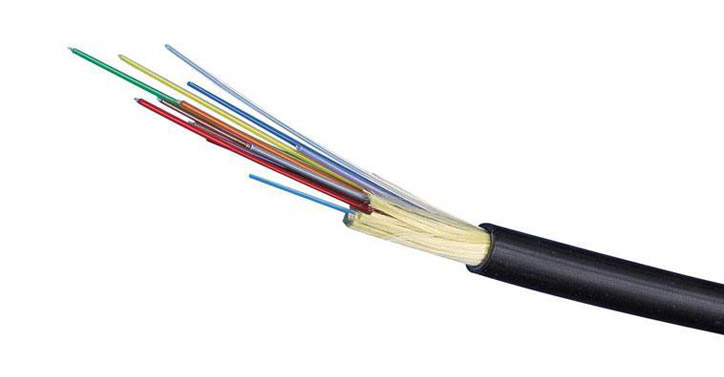
\includegraphics[width=0.6\linewidth]{img/om4.jpeg}
    \caption{Cáp quang OM4}
\end{figure}

\begin{itemize}[left=2cm]
    \item Hỗ trợ tốc độ từ 10Gbps trong khoảng cách tối đa là 550m, và tốc độ có thể đạt đến 100Gbps trong khoảng cách 100m.
    \item Sử dụng để kết nối giữa Switch Core -> Switch Distribution, Router -> Firewall, và Router -> ISP.
\end{itemize}

$-$ Cáp Cat6a
\begin{figure}[htbp]
    \centering    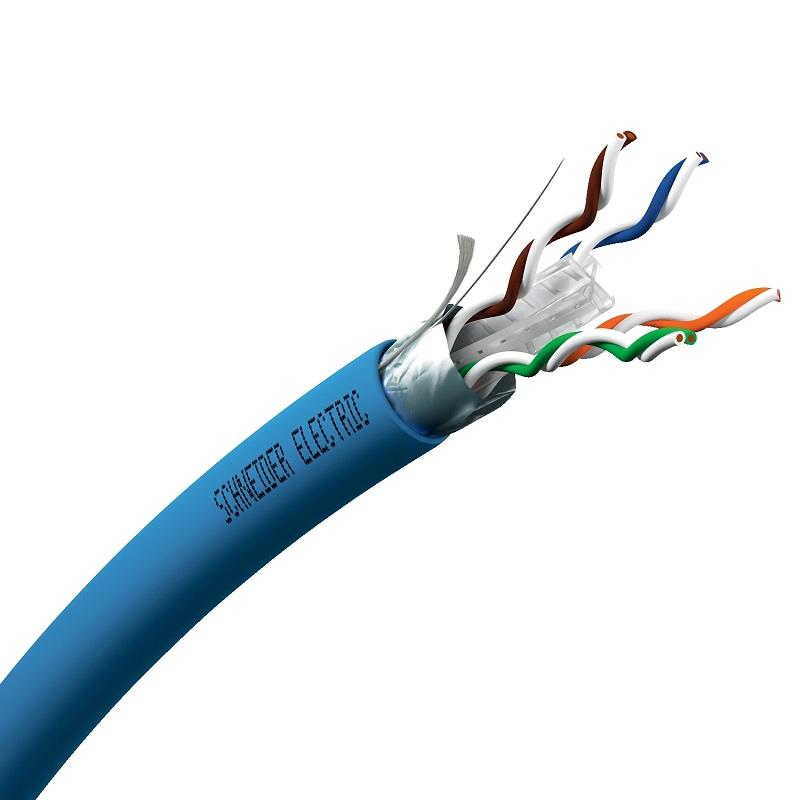
\includegraphics[width=0.5\linewidth]{img/cat6a.jpeg}
    \caption{Cáp quang Cat6a}
\end{figure}

\begin{itemize}[left=2cm]
    \item Hỗ trợ tốc độ từ 10Gbps trong khoảng cách tối đa là 100m.
    \item Sử dụng để kết nối từ Switch đến các thiết bị đầu cuối.
\end{itemize}

\section*{2.3 Sơ đồ luận lý}
\addcontentsline{toc}{section}{2.3 Sơ đồ luận lý}
\begin{figure}[htbp]
    \centering
    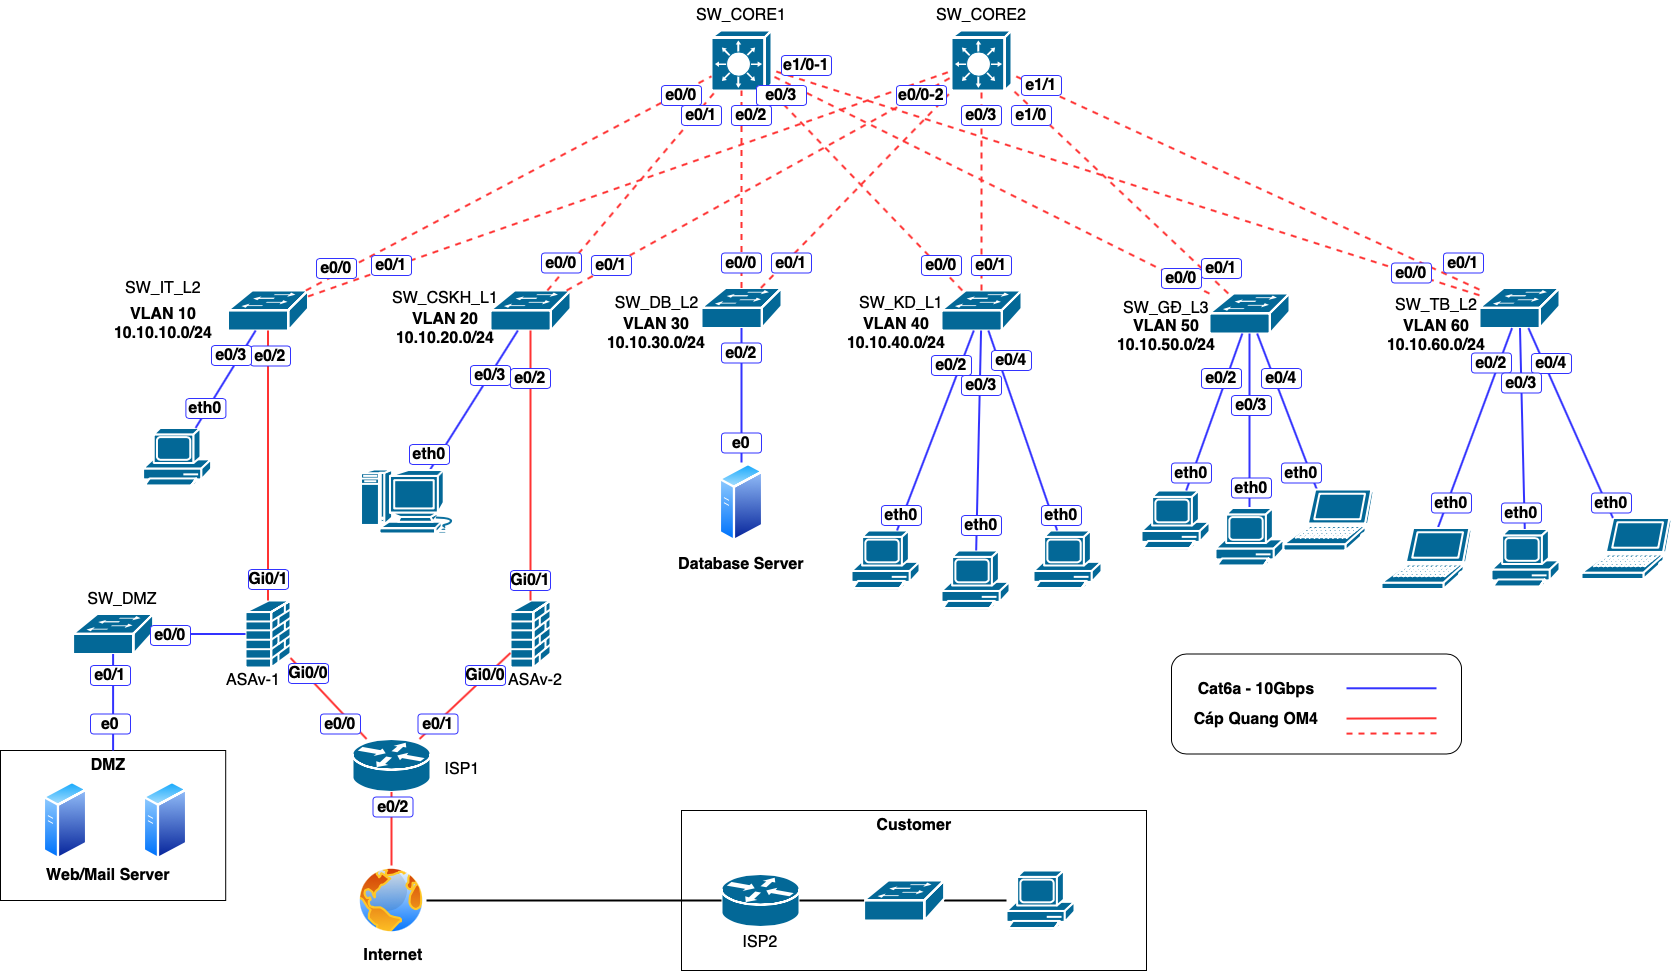
\includegraphics[width=1\linewidth]{img/logicFinalExam.png}
    \caption{Sơ đồ luận lý của hệ thống}
\end{figure}

\textbf{Mô tả:} Sơ đồ logic này mô tả một mạng nội bộ phức tạp nhưng tối ưu với cấu trúc phân chia VLAN, khu vực DMZ cách ly, hệ thống máy chủ và kết nối Internet thông qua các tầng bảo mật và tốc độ cao.

\textbf{Chi tiết thiết bị:}
\begin{itemize}[left=2cm]
    \item \textbf{Router}: Kết nối các VLAN với nhau, định tuyến lưu lượng mạng từ bên ngoài và trong nội bộ.
    \item \textbf{Firewall}: Bảo vệ mạng nội bộ, kiểm soát lưu lượng ra/vào. Tách biệt khu vực DMZ với các hệ thống quan trọng bên trong.
    \item \textbf{Switch}: Kết nối các thiết bị trong cùng VLAN, phân chia và chuyển tiếp dữ liệu nội bộ.
    \item \textbf{Switch Core}: Là trung tâm kết nối các switch truy cập, xử lý lưu lượng lớn giữa các VLAN và thiết bị, đảm bảo hiệu suất mạng cao và ổn định.
    \item \textbf{Database Server}: Lưu trữ và xử lý dữ liệu quan trọng, đặt bên trong hệ thống để dữ liệu được bảo mật.
    \item \textbf{Các Server}: Cung cấp các dịch vụ như tên miền, web, email, DHCP,...được hoạt động trong khu vực DMZ.
    \item \textbf{Thiết bị cuối}: Wifi, máy tính, laptop các nhân, máy in, camera, màn hình máy chiếu,...phục vụ công việc hàng ngày trong công ty.
\end{itemize}

\begin{table}[htbp]
\centering
\begin{tabular}{|c|l|}
\hline
\textbf{VLANs }& \textbf{Mô tả} \\
\hline
VLAN 10 & Dành cho bộ phận Kỹ thuật ở tầng 2 \\
\hline
VLAN 20 & Dành cho bộ phận CSKH ở tầng 1 \\
\hline
VLAN 30 & Dành cho máy Data server tại Trung tâm dữ liệu tầng 2\\
\hline
VLAN 40 & Dành cho bộ phận Kinh doanh ở tầng 1 \\
\hline
VLAN 50 & Dành cho phòng Giám đốc và Quản lý ở tầng 3 \\
\hline
VLAN 60 & Dành cho các thiết bị đầu cuối \\
\hline
VLAN 70 & Dành cho khu vực DMZ \\
\hline
\end{tabular}
\caption{Bảng mô tả VLAN ở SmartTech}
\end{table}

\textbf{Mục đích của sơ đồ logic:}
\begin{itemize}[left=2cm]
    \item Phân chia mạng hợp lý bằng VLAN: Tách biệt các bộ phận hoặc nhóm công việc (như kỹ thuật, kinh doanh, lãnh đạo) để tối ưu hóa hiệu suất và bảo mật.
    \item Đảm bảo bảo mật: DMZ bảo vệ các máy chủ quan trọng khỏi các mối đe dọa bên ngoài. Ngoài ra, Cách ly Database Server khỏi các thiết bị đầu cuối để giảm nguy cơ truy cập trái phép.
    \item Tăng hiệu suất mạng: Sử dụng VLAN giúp giảm thiểu xung đột mạng và đảm bảo lưu lượng truy cập không bị tắc nghẽn. Kết nối bằng cáp tốc độ cao như Cat6a, OM4 đảm bảo truyền dữ liệu nhanh và ổn định.
    \item Quản lý dễ dàng: Phân chia rõ ràng các khu vực mạng giúp quản trị viên dễ dàng quản lý, giám sát và khắc phục sự cố.
    \item Tăng tính linh hoạt và khả năng mở rộng: Cấu trúc này cho phép bổ sung thiết bị hoặc mở rộng mạng mà không ảnh hưởng đến hệ thống hiện tại.
    \item Kết nối với công ty khách hàng: Hệ thống được thiết kế để vừa hỗ trợ giao tiếp nội bộ, vừa kết nối với công ty khách hàng dễ dàng và hiệu quả.
\end{itemize}
\section*{2.4 Sơ đồ vật lý}
\addcontentsline{toc}{section}{2.4 Sơ đồ vật lý}
\subsection*{2.4.1 Sơ đồ bố trí}
\addcontentsline{toc}{subsection}{2.4.1 Sơ đồ bố trí}

\textbf{\textit{Sơ đồ vật lý tổng quát}}
\begin{figure}[htbp]
    \centering
    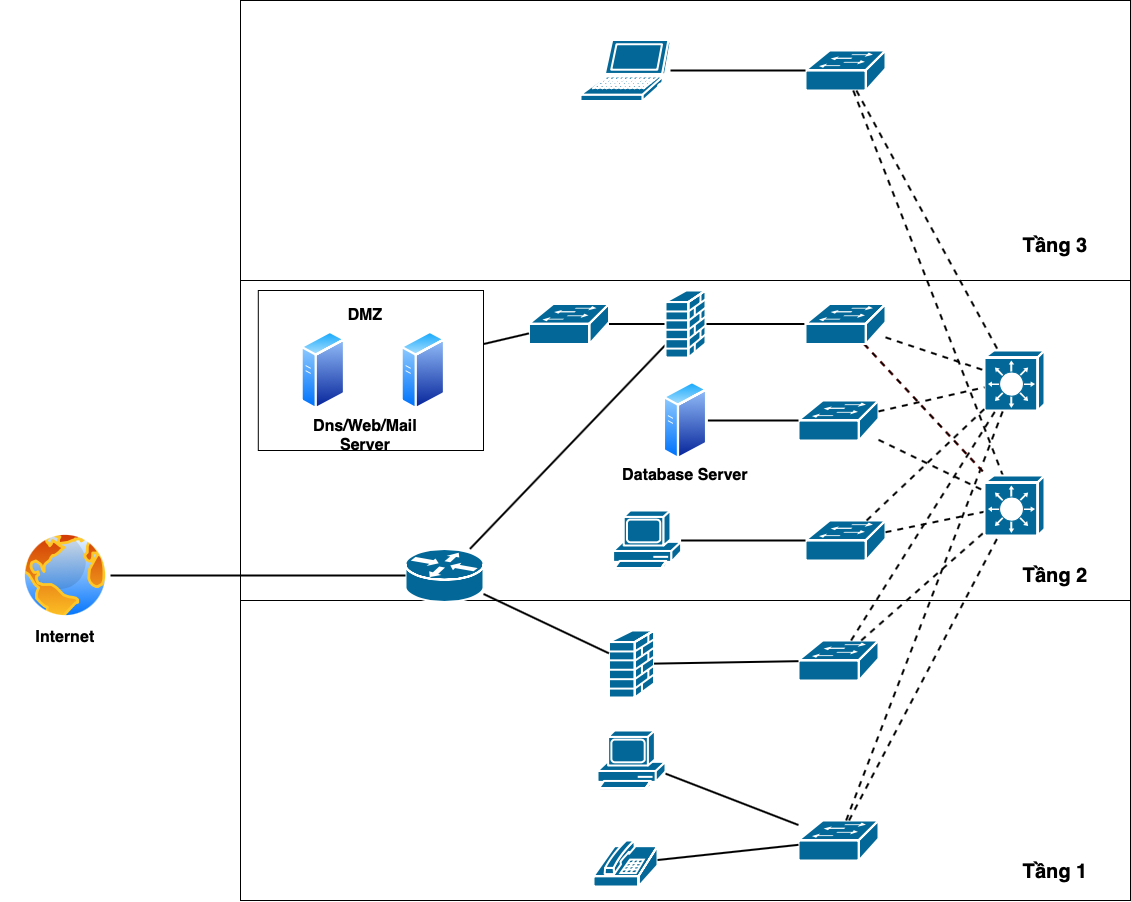
\includegraphics[width=0.8\linewidth]{img/physicOverview.png}
    \caption{Tổng quát vị trí các thiết bị trong hệ thống}
\end{figure}
\newpage

\textbf{\textit{Sơ đồ vật lý đi cáp từng tầng}}

$-$ Tầng 1:

\begin{figure}[htbp]
    \centering
    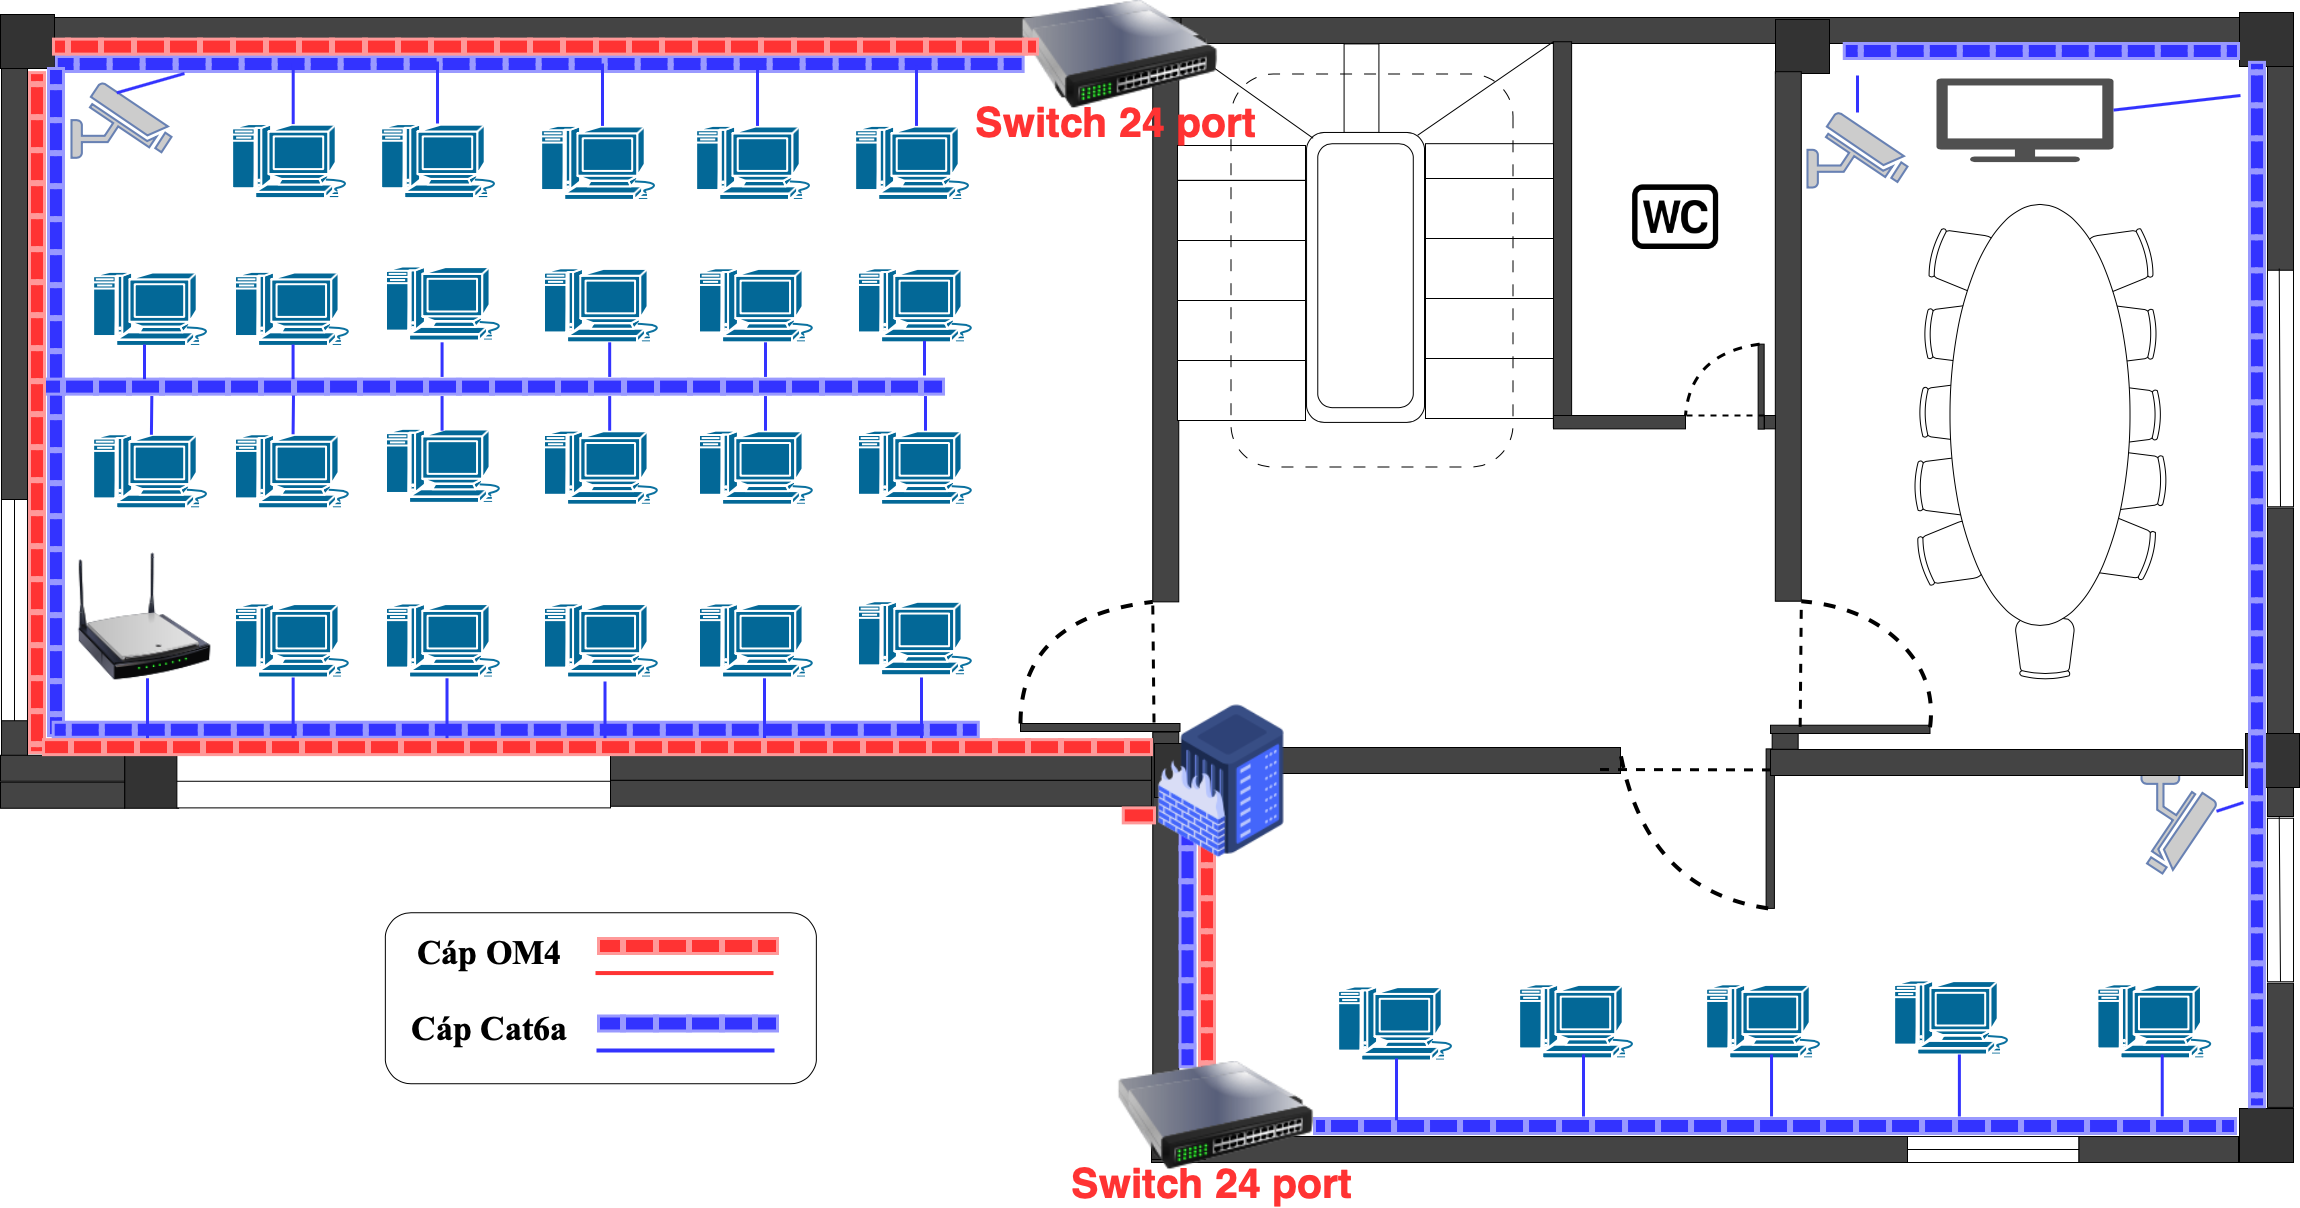
\includegraphics[width=1\linewidth]{img/floor1-2.png}
    \caption{Vị trí đi cáp và thiết bị tầng 1}
\end{figure}

$-$ Tầng 2:

\begin{figure}[htbp]
    \centering
    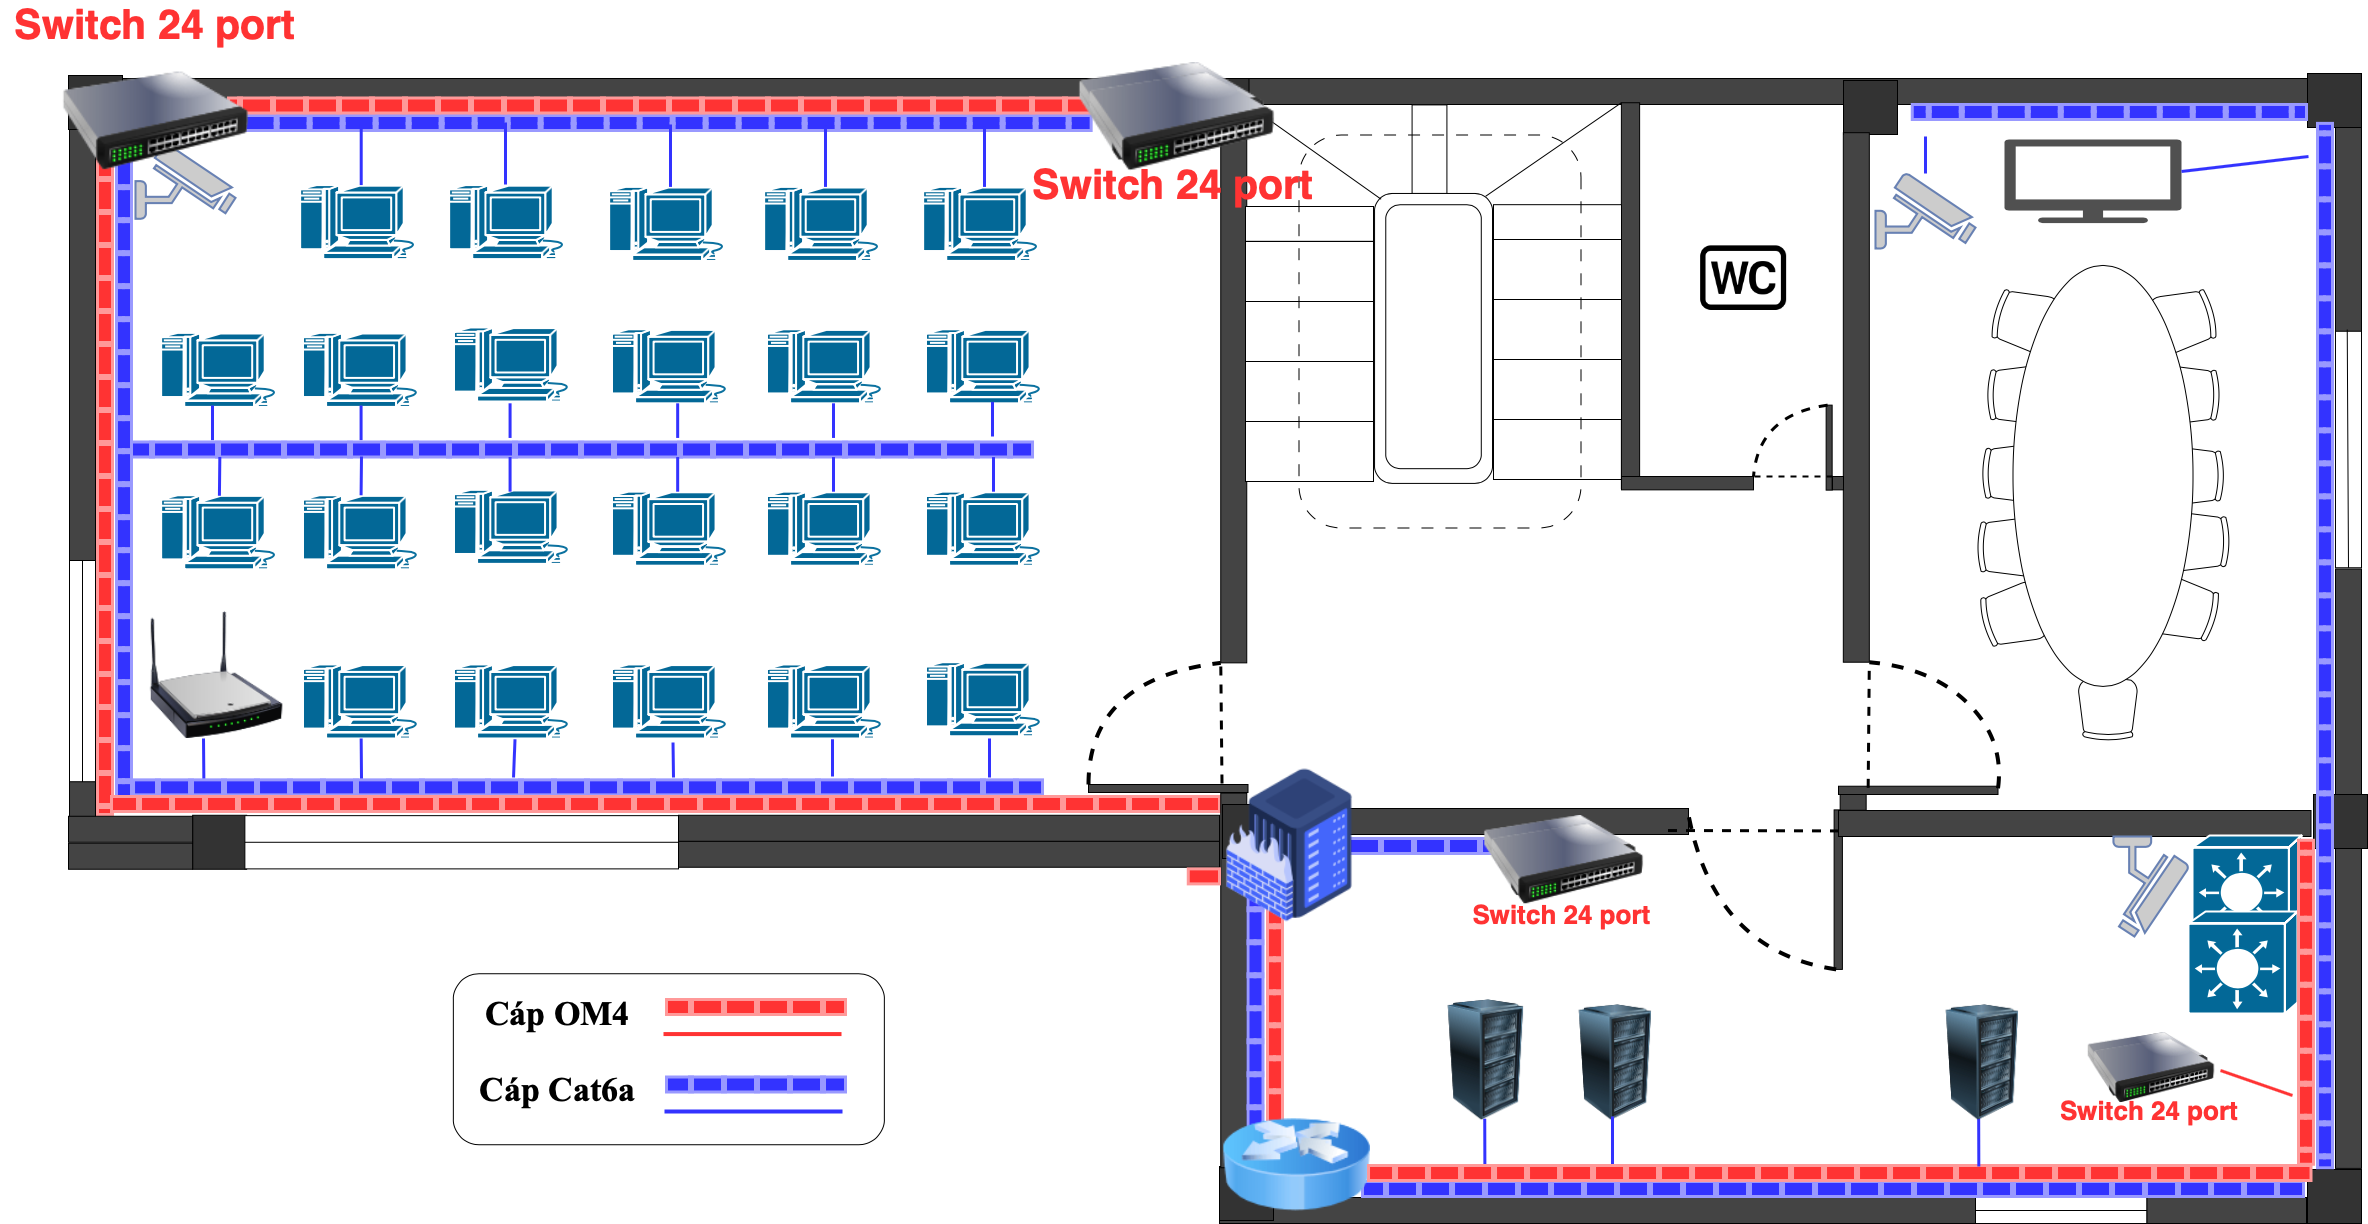
\includegraphics[width=1\linewidth]{img/floor2-2.png}
    \caption{Vị trí đi cáp và thiết bị tầng 2}
\end{figure}
\newpage
$-$ Tầng 3:

\begin{figure}[htbp]
    \centering
    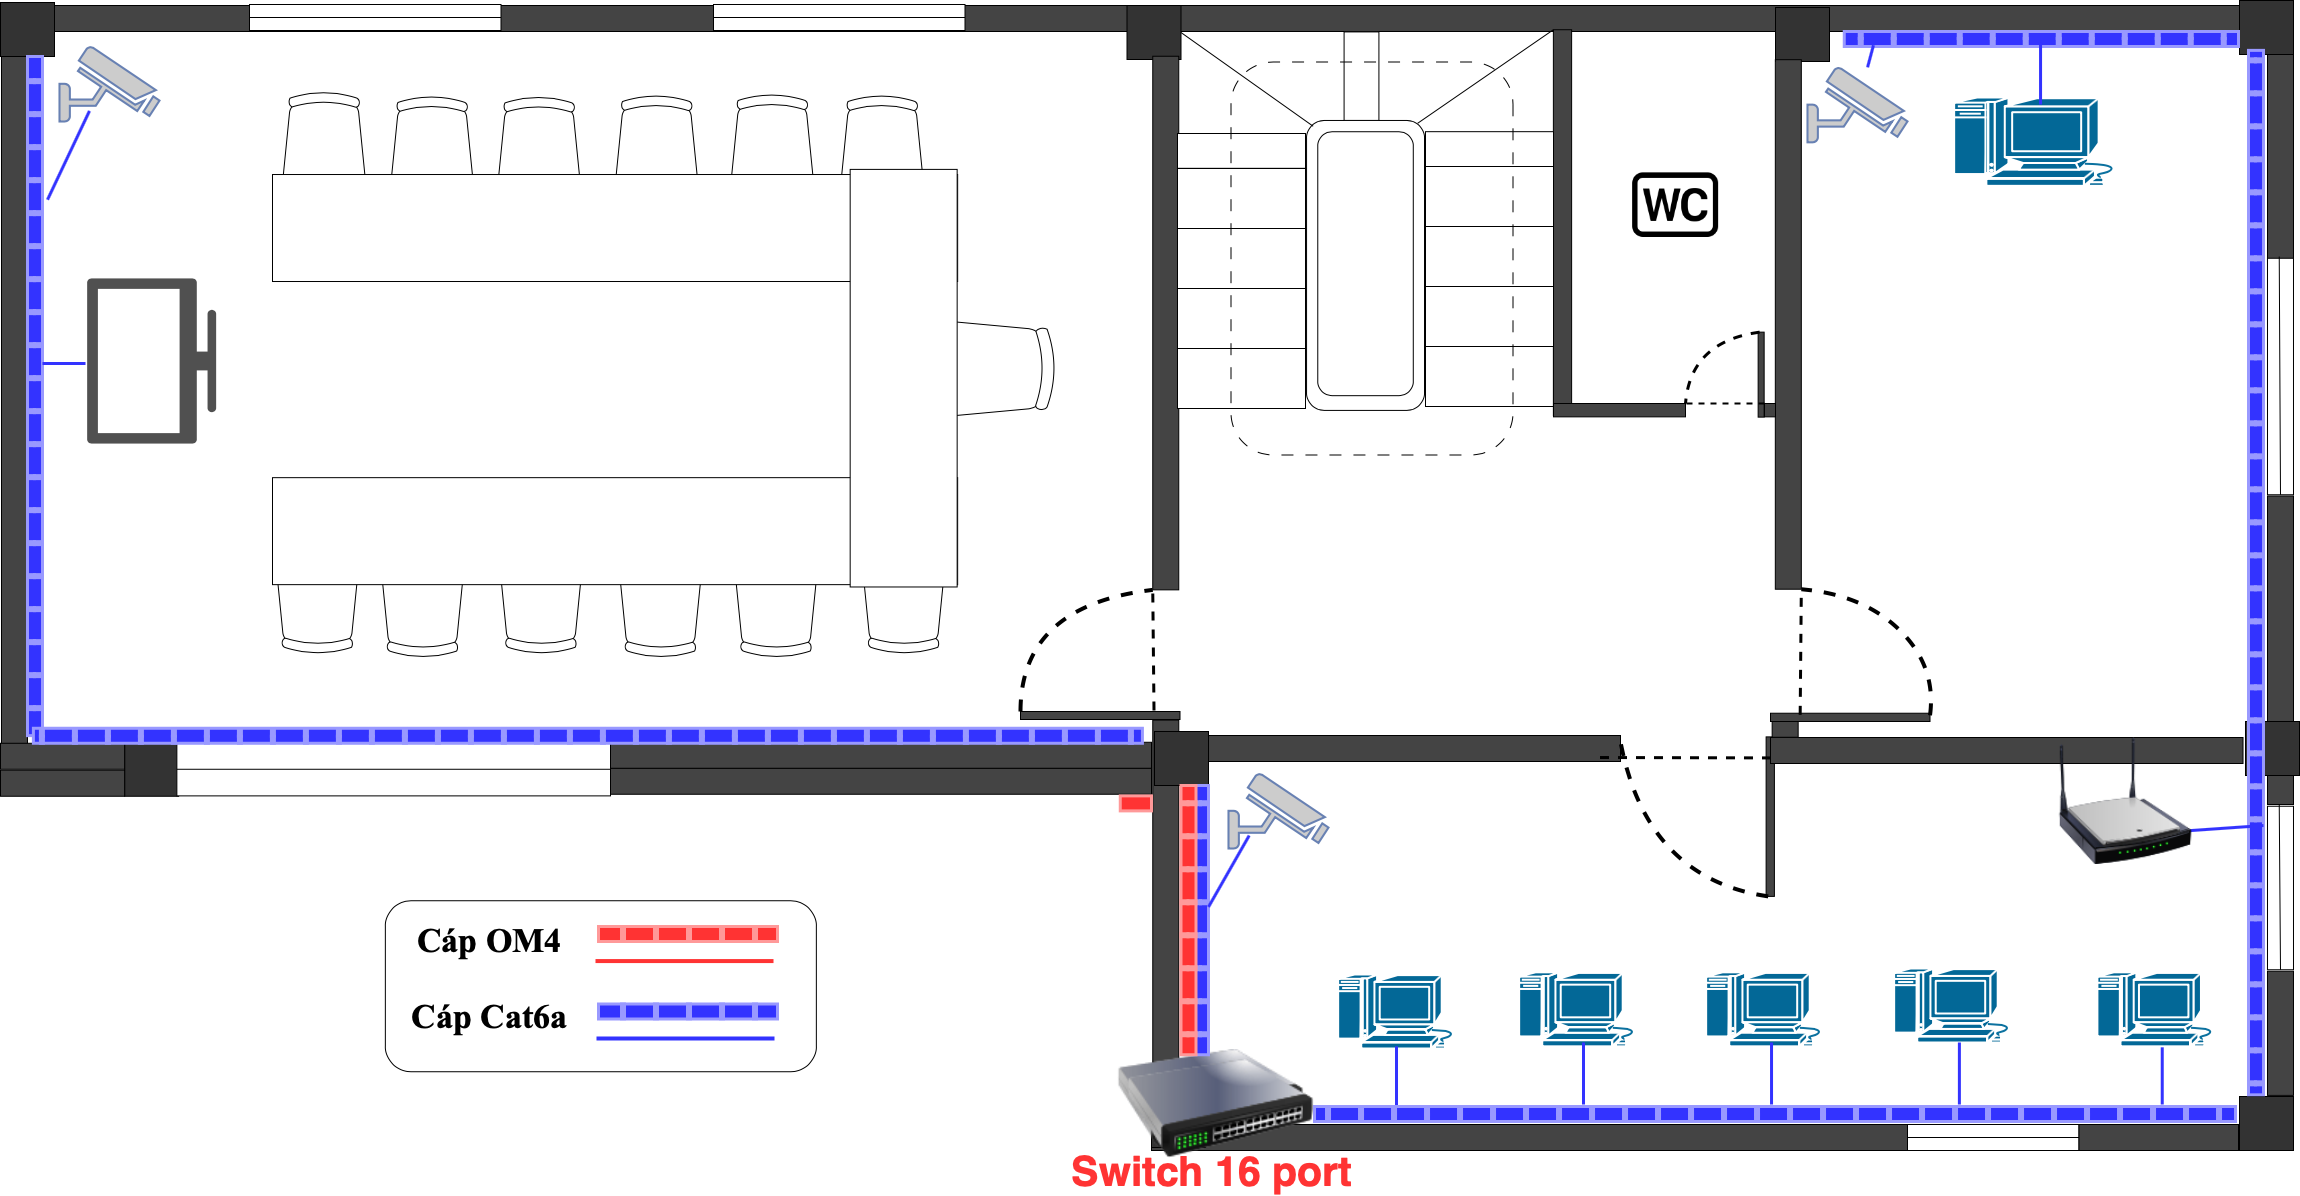
\includegraphics[width=1\linewidth]{img/floor3-2.png}
    \caption{Vị trí đi cáp và thiết bị tầng 3}
\end{figure}

Trong quá trình thiết kế, nhiều yếu tố được xem xét và thực hiện cẩn thận để đảm bảo hiệu suất, tin cậy của hệ thống:
\begin{itemize}
    \item \textbf{Sử dụng mô hình dạng sao:} Mô hình này đảm bảo được lưu lượng truyền dẫn mà không bị gián đoạn. Giúp dễ dàng sửa chữa và bảo trì khi gặp sự cố thiết bị.
    \item \textbf{Cấp điện áp:} Lựa chọn cấp điện áp phù hợp với yêu cầu hệ thống và xác định nguồn điện chính để đáp ứng nhu cầu sử dụng.
    \item \textbf{Điện dung máy biến áp:} Chọn máy biến áp có công suất phù hợp với phụ tải thực tế, đảm bảo hiệu suất hoạt động tối ưu.
    \item \textbf{Tiết diện dây dẫn:} Tính toán tiết diện dây dẫn đủ chịu tải và giảm thiểu tổn thất điện năng.
    \item \textbf{Phân bố trạm phân phối:} Bố trí trạm phân phối hợp lý để đảm bảo hiệu quả cung cấp điện cho các thiết bị và phụ tải.
    \item \textbf{Nguồn điện dự phòng:} Lắp đặt máy phát điện công nghiệp để duy trì cấp điện liên tục khi mất nguồn chính.
    \item \textbf{Đi dây cáp:} Sắp xếp dây cáp gọn gàng, sử dụng ống bảo vệ và thiết kế đi dây ẩn để dễ bảo trì và đảm bảo thẩm mỹ.
\end{itemize}
\subsection*{2.4.2 Các thiết bị sự dụng và chi phí dự kiến}
\addcontentsline{toc}{subsection}{2.4.2 Các thiết bị sự dụng và chi phí dự kiến }

\begin{table}[htbp]
\centering
\begin{tabular}{|c|l|c|r|r|}
\hline
\textbf{Loại thiết bị} &\textbf{Tên thiết bị} & \textbf{Số lượng} & \textbf{Giá thành (VND)} & \textbf{Tổng chi phí (VND)} \\
\hline
Router & CISCO ISR4221/K9 & 1 & 16.300.000 & 16.300.000\\
\hline
Switch & CISCO Catalyst 2960-X (24 port)& 6 & 54.500.000 & 327.000.000 \\
\hline
Switch & CISCO SG-95-16 (16 port) & 1 & 3.450.000 & 3.450.000\\
\hline
Switch Core & CISCO NEXUS 93180YC-EX & 2 & 28.000.000 & 56.000.000 \\
\hline
Firewall & CISCO ASA5516-FPWR-K9 & 2 & 69.500.000 & 139.000.000 \\
\hline
Server & Dell EMC PowerEdge R740XD & 3 & 72.800.000 & 218.400.000 \\
\hline
Máy tính & Máy tính để bàn & 80 & 10.000.000 & 800.000.000 \\
\hline
Dây cáp & Cáp quang OM4 & &  &  \\
\hline
Dây cáp & Cáp Cat6A &  &  & \\
\hline
\multicolumn{3}{|l|}{\textbf{Tổng chi phí (dự kiến)}} & \multicolumn{2}{r|}{\textbf{1.560.150.000 VND}} \\
\hline
\end{tabular}
\caption{Thiết bị mạng và chi phí dự kiến}
\end{table}

\section*{2.5 Thông tin cài đặt cấu hình}
\addcontentsline{toc}{section}{2.5 Thông tin cài đặt cấu hình}

\subsection*{2.5.1 Thông tin VLAN trong hệ thống}
\addcontentsline{toc}{subsection}{2.5.1 Thông tin VLAN trong hệ thống}

\begin{table}[htbp]
\centering
\begin{tabular}{|c|l|c|l|c|c|}
\hline
\textbf{VLAN} & \textbf{Tên VLAN} & \textbf{VXLAN} &\textbf{Mô tả }& \textbf{Network} & \textbf{Default Gateway} \\
\hline
1 & Management &-& VLAN mặc định & 10.10.1.0/24 & 10.10.10.254\\
\hline
10 & KyThuat & 1010&Dành cho ban Kỹ thuật ở tầng 2 & 10.10.10.0/24 & 10.10.20.254\\
\hline
20 & CSKH & 1020& Dành cho ban CSKH ở tầng 1 & 10.10.20.0/24 & 10.10.20.254\\
\hline
30 & TTDL & 1030&Dành cho Trung tâm dữ liệu tầng 2 & 10.10.30.0/24 & 10.10.30.254\\
\hline
40 & KinhDoanh & 1040&Dành cho ban Kinh doanh ở tầng 1 & 10.10.40.0/24 & 10.10.40.254\\
\hline
50 & GiamDoc &1050& Dành cho phòng Giám đốc tầng 3& 10.10.50.0/24 & 10.10.50.254\\
\hline
60 & ThietBi &1060&Dành cho các thiết bị đầu cuối & 10.10.60.0/24 & 10.10.60.254\\
\hline
70 & DMZ & - &Dành cho khu vực DMZ & 10.10.70.0/24 & 10.10.70.1\\
\hline
\end{tabular}
\caption{Thông tin chi tiết VLAN trong mô hình mạng}
\end{table}
\newpage

\subsection*{2.5.2 Thông tin kết nối port trong hệ thống}
\addcontentsline{toc}{subsection}{2.5.2 Thông tin kết nối port trong hệ thống}

\begin{table}[htbp]
\centering
\begin{tabular}{|c|c|c|c|c|}
\hline
\multicolumn{2}{|c|}{\textbf{Source}} & \multicolumn{2}{c|}{\textbf{Destination}} & \textbf{Trunking/ }\\
\cline{1-4}
\textbf{Tên thiết bị} & \textbf{Interface} & \textbf{Interface} & \textbf{Tên thiết bị} & \textbf{VLAN}\\
\hline
IPS1 & e0/0 & Gi0/0 & ASAv-1 & -\\
\hline
IPS1 & e0/1 & Gi0/0 & ASAv-2 & -\\
\hline
ASAv-1 & Gi0/1 &  e0/2 & SW-IT-L2 & -\\
\hline
ASAv-1 & Gi0/2 &  e0/0 & SW-DMZ & -\\
\hline
SW-DMZ& e0/1 &  e0 & Web/Mail Server & -\\
\hline
ASAv-2& Gi0/1 &  e0/2 & SW-CSKH-L1 & -\\
\hline
SW-CORE1 & e0/0  & e0/0 & SW-IT-L2 & -\\
\hline
SW-CORE1 & e0/1  & e0/0 & SW-CSKH-L1 & -\\
\hline
SW-CORE1 & e0/2  & e0/0 & SW-DB-L2 & -\\
\hline
SW-CORE1 & e0/3  & e0/0 & SW-KD-L2 & -\\
\hline
SW-CORE1 & e1/0  & e0/0 & SW-GĐ-L3 & -\\
\hline
SW-CORE1 & e1/1  & e0/0 & SW-TB-L2 & -\\
\hline
SW-CORE2 & e0/0  & e0/1 & SW-IT-L2 & -\\
\hline
SW-CORE2 & e0/1  & e0/1 & SW-CSKH-L1 & -\\
\hline
SW-CORE2 & e0/2  & e0/1 &SW-DB-L2 & -\\
\hline
SW-CORE2 & e0/3  & e0/1 & SW-KD-L2& -\\
\hline
SW-CORE2 & e1/0  & e0/1 & SW-GĐ-L3 & -\\
\hline
SW-CORE2 & e1/1  & e0/1 & SW-TB-L2 & -\\
\hline
SW-DB-L2 & e0/2  & e0 & Database Server & VLAN 30\\
\hline
 SW-IT-L2& e0/3  & eth0 & PC & VLAN 10\\
\hline
SW-CSKH-L1 & e0/3  & eth0 & PC & VLAN 20\\
\hline
SW-KD-L1 & e0/2  & eth0 & PC & VLAN 40\\
\hline
SW-KD-L1 & e0/3  & eth0 & PC & VLAN 40\\
\hline
SW-KD-L1 & e0/4  & eth0 & PC & VLAN 40\\
\hline
SW-GĐ-L3 & e0/2  & eth0 & PC & VLAN 50\\
\hline
SW-GĐ-L3 & e0/3  & eth0 & PC & VLAN 50\\
\hline
SW-GĐ-L3 & e0/4  & eth0 & PC & VLAN 50\\
\hline
SW-TB-L2 & e0/2  & eth0 & PC & VLAN 60\\
\hline
SW-TB-L2 & e0/3  & eth0 & PC & VLAN 60\\
\hline
SW-TB-L2 & e0/4  & eth0 & PC & VLAN 60\\
\hline
\end{tabular}
\caption{Thông tin kết nối port trong hệ thống}
\end{table}
\newpage
\subsection*{2.5.3 Thông tin quy hoạch địa chỉ IP}
\addcontentsline{toc}{subsection}{2.5.3 Thông tin quy hoạch địa chỉ IP}

\begin{table}[htbp]
\centering
\begin{tabular}{|c|l|c|c|c|}
\hline
\textbf{Name} & \textbf{Interface} & \textbf{Subnet} & \textbf{IP} & \textbf{Neighbor} \\
\hline
\multirow{6}{*}{Core-1} & Ethernet0/0 & 192.168.1.0/30 & 192.168.1.1 & 192.168.1.2 \\
\cline{2-5}
& Ethernet0/1 & 192.168.1.4/30 & 192.168.1.5 & 192.168.1.6 \\
\cline{2-5}
& Ethernet0/2 & 192.168.1.8/30 & 192.168.1.9 & 192.168.1.10 \\
\cline{2-5}
& Ethernet0/3 & 192.168.1.12/30 & 192.168.1.13 & 192.168.1.14 \\
\cline{2-5}
& Ethernet1/0 & 192.168.1.16/30 & 192.168.1.17 & 192.168.1.18 \\
\cline{2-5}
& Ethernet1/1 & 192.168.1.20/30 & 192.168.1.21 & 192.168.1.22 \\
\hline
\multirow{6}{*}{Core-2} & Ethernet0/0 & 192.168.1.24/30 & 192.168.1.25 & 192.168.1.26 \\
\cline{2-5}
& Ethernet0/1 & 192.168.1.28/30 & 192.168.1.29 & 192.168.1.30 \\
\cline{2-5}
& Ethernet0/2 & 192.168.1.32/30 & 192.168.1.33 & 192.168.1.34 \\
\cline{2-5}
& Ethernet0/3 & 192.168.1.36/30 & 192.168.1.37 & 192.168.1.38 \\
\cline{2-5}
& Ethernet1/0 & 192.168.1.40/30 & 192.168.1.41 & 192.168.1.42 \\
\cline{2-5}
& Ethernet1/1 & 192.168.1.44/30 & 192.168.1.45 & 192.168.1.46 \\
\hline
DNS Server &Ethernet0/0  & 10.10.70.0/24 &10.10.70.10 & 10.10.70.1 \\
\hline
Mail Server &Ethernet0/0  & 10.10.70.0/24 &10.10.70.11 & 10.10.70.1 \\
\hline
Database Server &Ethernet0/2& 10.10.30.0/24 &10.10.30.10 & 10.10.30.1 \\
\hline
Máy PC tại phòng KD &Eth0/2 - Eth6/2  & 10.10.40.0/26 &10.10.40.1 - 10.10.40.62 &10.10.40.1 \\
\hline
Máy PC tại phòng CSKH &Eth0/3 - Eth3/0  & 10.10.20.0/27 &10.10.20.1 - 10.10.20.30 & 10.10.20.1 \\
\hline
Máy PC tại phòng KT &Eth0/3 - Eth10/2  & 10.10.10.0/26 &10.10.10.1 - 10.10.10.62 & 10.10.10.1 \\
\hline
Máy PC tại phòng GĐ &Eth0/2 - Eth1/2  & 10.10.50.0/29 &10.10.50.1 - 10.10.50.6 & 10.10.50.1 \\
\hline
Máy chiếu,camera,máy in&Eth0/2 - Eth4/0  & 10.10.60.0/26 &10.10.60.1 - 10.10.60.62 &10.10.60.1 \\
\hline
\end{tabular}
\caption{Quy hoạch địa chỉ IP}
\label{tab:network-config}
\end{table}

Yêu cầu về số lượng địa chỉ IP (mở rộng 50\% trong tương lai):

- \textit{Phòng Kinh doanh:} Có 25 nhân viên

\begin{center}
    25 + (25 × 50\%) = 38
\end{center}

=> Cần tối thiểu 38 IP, do đó nên chọn subnet có khả năng chứa ít nhất 38 IP, chọn 10.10.40.0/26.

- \textit{Phòng CSKH:} Có 10 nhân viên

\begin{center}
    10 + (10 × 50\%) = 15
\end{center}

=> Cần tối thiểu 15 IP, do đó nên chọn subnet có khả năng chứa ít nhất 15 IP, chọn 10.10.20.0/27.

- \textit{Phòng Kỹ thuật:} Có 40 nhân viên

\begin{center}
    40 + (40 × 50\%) = 60
\end{center}

=> Cần tối thiểu 60 IP, do đó nên chọn subnet có khả năng chứa ít nhất 60 IP, chọn 10.10.10.0/26.

- \textit{Phòng Kinh doanh:} Có 5 người gồm 4 quản lý và 1 giám đốc.

=> Cần tối thiểu 5 IP, do đó nên chọn subnet có khả năng chứa ít nhất 5 IP, chọn 10.10.50.0/29.

- \textit{Các thiết bị:} Dự phòng khoảng 20-30 thiết bị 

=> Cần tối thiểu 30 IP, do đó nên chọn subnet có khả năng chứa ít nhất 30 IP, chọn 10.10.60.0/27.

Kết luận:
\begin{itemize}[left=2cm]
    \item Quy hoạch này đảm bảo phòng KD, CSKH, và KT có đủ địa chỉ IP hiện tại và khả năng mở rộng 50\% trong tương lai.
    \item Subnet được tối ưu hóa, hạn chế lãng phí không gian địa chỉ IP, đồng thời phù hợp với nhu cầu thực tế của từng phòng ban.
\end{itemize}
